\documentclass[conference]{IEEEtran}
\IEEEoverridecommandlockouts
% The preceding line is only needed to identify funding in the first footnote. If that is unneeded, please comment it out.
\usepackage{cite}
\usepackage{amsmath,amssymb,amsfonts}
\usepackage{algorithmic}
\usepackage{graphicx}
\usepackage{textcomp}
\usepackage{xcolor}
\usepackage{hyperref}
\usepackage{enumerate}  %枚举的符号
\usepackage{geometry}   %页面形式
\usepackage{fancyhdr}   % 设置页眉
\usepackage{xcolor} %颜色
\usepackage{listings}   %插入代码
\usepackage{amsmath}
\usepackage{mathtools}
\usepackage{amsthm}
\usepackage{amssymb}
\usepackage{amsfonts}
\usepackage{longtable}  %长表格
\usepackage[all,cmtip]{xy}  %交换图
\usepackage{pgf,tikz}   %自动机画图
\usetikzlibrary{shapes,arrows,automata}
\usepackage{graphicx}

% \usepackage{algorithm}  %算法
% \usepackage{algpseudocode}
\usepackage{graphics}
\usepackage{epsfig}
%算法中用\require, \ensure写input,output
% \renewcommand{\algorithmicrequire}{\textbf{Input:}} % Use Input in the format of Algorithm
% \renewcommand{\algorithmicensure}{\textbf{Output:}} % Use Output in the format of Algorithm
% \newcommand{\algorithmiclastcon}{\textbf{Initialize:}}
% \newcommand{\Initialize}{\item[\algorithmiclastcon]}

\usepackage{framed} %给文字加框

\usepackage{bm} %给数学公式中的符号加粗
\usepackage{bbm}

\usepackage{yhmath} %把\Widehat命令设为自动调整大小的hat符号
\DeclareSymbolFont{largesymbol}{OMX}{yhex}{m}{n}
\DeclareMathAccent{\Widehat}{\mathord}{largesymbol}{"62}

\renewcommand\tablename{Table}  %设置图表的名字
\renewcommand\figurename{Figure}
% \CTEXoptions[today=old] %设置日期为英文
\renewcommand\refname{Reference}    % 设置参考文献为英文

\setlength{\parindent}{0pt} %设置不缩进
\linespread{1}  % 改变行距

% \usepackage[T1]{fontenc} %  textsc
\usepackage{xspace}
\usepackage{enumitem}

\usepackage{todonotes}

\usepackage{multirow}
\usepackage{booktabs}





\newtheorem{problem}{Problem}
\newtheorem{lemma}{Lemma}
\newtheorem{theorem}[lemma]{Theorem}
\newtheorem{corollary}[lemma]{Corollary}
\newtheorem{proposition}[lemma]{Proposition}
\newtheorem{definition}[lemma]{Definition}
\newtheorem{property}{Property}
\newtheorem{assumption}{Assumption}
\newtheorem{conjecture}{Conjecture}
\newtheorem*{exercise}{Exercise}
\newtheorem*{remark}{Remark}
\newtheorem*{observation}{Observation}
\newtheorem*{example}{Example}
\newtheorem*{solution}{Solution}
\newtheorem*{notation}{Notation}
\newtheorem*{question}{Question}
% \newtheorem*{conjecture}{Conjecture}


% notations
\newcommand{\wt}[1]{\widetilde{#1}}
\newcommand{\h}[1]{\Widehat{#1}}
\renewcommand{\o}[1]{\overline{#1}}
\renewcommand{\u}[1]{\underline{#1}}
\newcommand{\s}[1]{\sqrt{#1}}
\renewcommand{\d}{\textnormal{d}}
\newcommand{\tto}{\Rightarrow}


% formatting
\newcommand\blankline{~\\}



\newcommand{\cA}{\mathcal{A}}
\newcommand{\cB}{\mathcal{B}}
\newcommand{\cC}{\mathcal{C}}
\newcommand{\cD}{\mathcal{D}}
\newcommand{\cE}{\mathcal{E}}
\newcommand{\cF}{\mathcal{F}}
\newcommand{\cG}{\mathcal{G}}
\newcommand{\cH}{\mathcal{H}}
\newcommand{\cI}{\mathcal{I}}
\newcommand{\cJ}{\mathcal{J}}
\newcommand{\cK}{\mathcal{K}}
\newcommand{\cL}{\mathcal{L}}
\newcommand{\cM}{\mathcal{M}}
\newcommand{\cN}{\mathcal{N}}
\newcommand{\cO}{\mathcal{O}}
\newcommand{\cP}{\mathcal{P}}
\newcommand{\cQ}{\mathcal{Q}}
\newcommand{\cR}{\mathcal{R}}
\newcommand{\cS}{\mathcal{S}}
\newcommand{\cT}{\mathcal{T}}
\newcommand{\cU}{\mathcal{U}}
\newcommand{\cV}{\mathcal{V}}
\newcommand{\cW}{\mathcal{W}}
\newcommand{\cX}{\mathcal{X}}
\newcommand{\cY}{\mathcal{Y}}
\newcommand{\cZ}{\mathcal{Z}}




\newcommand{\bA}{\mathbb{A}}
\newcommand{\bB}{\mathbb{B}}
\newcommand{\bC}{\mathbb{C}}
\newcommand{\bD}{\mathbb{D}}
\newcommand{\bE}{\mathbb{E}}
\newcommand{\bF}{\mathbb{F}}
\newcommand{\bG}{\mathbb{G}}
\newcommand{\bH}{\mathbb{H}}
\newcommand{\bI}{\mathbb{I}}
\newcommand{\bJ}{\mathbb{J}}
\newcommand{\bK}{\mathbb{K}}
\newcommand{\bL}{\mathbb{L}}
\newcommand{\bM}{\mathbb{M}}
\newcommand{\bN}{\mathbb{N}}
\newcommand{\bO}{\mathbb{O}}
\newcommand{\bP}{\mathbb{P}}
\newcommand{\bQ}{\mathbb{Q}}
\newcommand{\bR}{\mathbb{R}}
\newcommand{\bS}{\mathbb{S}}
\newcommand{\bT}{\mathbb{T}}
\newcommand{\bU}{\mathbb{U}}
\newcommand{\bV}{\mathbb{V}}
\newcommand{\bW}{\mathbb{W}}
\newcommand{\bX}{\mathbb{X}}
\newcommand{\bY}{\mathbb{Y}}
\newcommand{\bZ}{\mathbb{Z}}




\newcommand{\va}{\mathbf{a}}
\newcommand{\vb}{\mathbf{b}}
\newcommand{\vc}{\mathbf{c}}
\newcommand{\vd}{\mathbf{d}}
\newcommand{\ve}{\mathbf{e}}
\newcommand{\vf}{\mathbf{f}}
\newcommand{\vg}{\mathbf{g}}
\newcommand{\vh}{\mathbf{h}}
\newcommand{\vi}{\mathbf{i}}
\newcommand{\vj}{\mathbf{j}}
\newcommand{\vk}{\mathbf{k}}
\newcommand{\vl}{\mathbf{l}}
\newcommand{\vm}{\mathbf{m}}
\newcommand{\vn}{\mathbf{n}}
\newcommand{\vo}{\mathbf{o}}
\newcommand{\vp}{\mathbf{p}}
\newcommand{\vq}{\mathbf{q}}
\newcommand{\vr}{\mathbf{r}}
\newcommand{\vs}{\mathbf{s}}
\newcommand{\vt}{\mathbf{t}}
\newcommand{\vu}{\mathbf{u}}
\newcommand{\vv}{\mathbf{v}}
\newcommand{\vw}{\mathbf{w}}
\newcommand{\vx}{\mathbf{x}}
\newcommand{\vy}{\mathbf{y}}
\newcommand{\vz}{\mathbf{z}}




\newcommand{\vA}{\mathbf{A}}
\newcommand{\vB}{\mathbf{B}}
\newcommand{\vC}{\mathbf{C}}
\newcommand{\vD}{\mathbf{D}}
\newcommand{\vE}{\mathbf{E}}
\newcommand{\vF}{\mathbf{F}}
\newcommand{\vG}{\mathbf{G}}
\newcommand{\vH}{\mathbf{H}}
\newcommand{\vI}{\mathbf{I}}
\newcommand{\vJ}{\mathbf{J}}
\newcommand{\vK}{\mathbf{K}}
\newcommand{\vL}{\mathbf{L}}
\newcommand{\vM}{\mathbf{M}}
\newcommand{\vN}{\mathbf{N}}
\newcommand{\vO}{\mathbf{O}}
\newcommand{\vP}{\mathbf{P}}
\newcommand{\vQ}{\mathbf{Q}}
\newcommand{\vR}{\mathbf{R}}
\newcommand{\vS}{\mathbf{S}}
\newcommand{\vT}{\mathbf{T}}
\newcommand{\vU}{\mathbf{U}}
\newcommand{\vV}{\mathbf{V}}
\newcommand{\vW}{\mathbf{W}}
\newcommand{\vX}{\mathbf{X}}
\newcommand{\vY}{\mathbf{Y}}
\newcommand{\vZ}{\mathbf{Z}}

\newcommand{\set}[1]{\{#1\}}
\newcommand{\Set}[1]{\left\{#1\right\}}
\newcommand{\inner}[1]{\langle#1\rangle}
\newcommand{\Inner}[1]{\left\langle#1\right\rangle}
\newcommand{\Var}{\textnormal{Var}}
\newcommand{\abs}[1]{\lvert#1\rvert}
\newcommand{\Abs}[1]{\left\lvert#1\right\rvert}
\newcommand{\norm}[1]{\left\|{#1}\right\|}
\newcommand{\Ot}{\widetilde{O}}


\newcommand{\bigSet}[1]{\bigl\{#1\bigr\}}
\newcommand{\BigSet}[1]{\Bigl\{#1\Bigr\}}
\newcommand{\braces}[1]{\{#1\}}
\newcommand{\Braces}[1]{\left\{#1\right\}}
\newcommand{\bigBraces}[1]{\bigl\{#1\bigr\}}
\newcommand{\BigBraces}[1]{\Bigl\{#1\Bigr\}}
\newcommand{\bracks}[1]{[#1]}
\newcommand{\Bracks}[1]{\left[#1\right]}
\newcommand{\bigBracks}[1]{\bigl[#1\bigr]}
\newcommand{\BigBracks}[1]{\Bigl[#1\Bigr]}
\newcommand{\biggBracks}[1]{\biggl[#1\biggr]}
\newcommand{\BiggBracks}[1]{\Biggl[#1\Biggr]}
\newcommand{\parens}[1]{(#1)}
\newcommand{\Parens}[1]{\left(#1\right)}
\newcommand{\bigParens}[1]{\bigl(#1\bigr)}
\newcommand{\BigParens}[1]{\Bigl(#1\Bigr)}
\newcommand{\biggParens}[1]{\biggl(#1\biggr)}
\newcommand{\BiggParens}[1]{\Biggl(#1\Biggr)}
\newcommand{\given}{\mathbin{\vert}}
\newcommand{\bigGiven}{\mathbin{\bigm\vert}}
\newcommand{\BigGiven}{\mathbin{\Bigm\vert}}
\newcommand{\biggGiven}{\mathbin{\biggm\vert}}

% \newcommand{\Mat}[1]{\begin\{pmatrix\}#1\end\{pmatrix\}}


\newcommand{\eps}{\epsilon}
\newcommand{\veps}{\varepsilon}


\newcommand{\wrong}[1]{\textcolor{red}{#1}}
\newcommand{\good}[1]{\textcolor{blue}{#1}}




\DeclareMathOperator*{\argmax}{arg\,max}
\DeclareMathOperator*{\argmin}{arg\,min}
\newcommand{\Ent}{\mathrm{Ent}}
\newcommand{\ERM}{\mathrm{ERM}}
\newcommand{\diam}{\mathrm{diam}}
\newcommand{\card}{\mathrm{card}}
\newcommand{\Unif}{\mathrm{Unif}}
\newcommand{\TV}{\mathrm{TV}}
\newcommand{\init}{\mathrm{init}}
\def\BibTeX{{\rm B\kern-.05em{\sc i\kern-.025em b}\kern-.08em
    T\kern-.1667em\lower.7ex\hbox{E}\kern-.125emX}}
\begin{document}

\title{Co-optimization\\
% {\footnotesize \textsuperscript{*}Note: Sub-titles are not captured in Xplore and
% should not be used}
% \thanks{Identify applicable funding agency here. If none, delete this.}
}

\author{
\IEEEauthorblockN{Yunsheng Tian}
\IEEEauthorblockA{\textit{Computer Science \& Artificial Intelligence Lab} \\
\textit{Massachusetts Institute of Technology}\\
Cambridge, MA 02139 \\
yunsheng@csail.mit.edu}
\and
\IEEEauthorblockN{Jian Qian}
\IEEEauthorblockA{Laboratory for Information \& Decision Systems \\
\textit{Massachusetts Institute of Technology}\\
Cambridge, MA 02139 \\
jianqian@mit.edu}
}

\maketitle

\begin{abstract}
We present a general scheme to co-optimize the control input and the robot design, where the target is to optimize the motion planning variables and the robot design parameters such as mass, length, etc., at the same time. The scheme includes two parts: the motion planning part and the parameter optimization part. The motion planning part can be any existing algorithm, we used mainly iterative linear quadratic regulator (iLQR). For the parameter optimization, we use vanilla gradient descent. We demonstrate our results on pendulum and acrobot environment, showing that this scheme will try to make the environment more controllable. 
\end{abstract}

\begin{IEEEkeywords}
Co-optimizing, Acrobot, Pendulum, iLQR
\end{IEEEkeywords}


\section{Introduction}

For a robot to achieve certain tasks successfully, we all know that control is important, but the design (i.e. structure) of the robot is important as well. So we want to simultaneously optimize for robot's control and design to figure out what's the best design of the robot for a given task and also the corresponding optimal policy for that design. The design of a robot along with its control determines the optimal performance for the robot to achieve certain tasks. But most of the previous works focus on improving robot control while the design optimization of robots is relatively less explored. Therefore, given certain tasks, we want to co-optimize both the design and the control of robots to achieve better performance than hand-designed robots. It would be also interesting to see how the optimal designs of robots look like and what insights we can get from the optimization.



\section{Related work}



\cite{spielberg2017functional} co-optimizes the design parameters of a robot and its trajectories.
\cite{ha2019reinforcement} explores a similar idea but uses DRL for control, and has the potential to work on more complex tasks.
\cite{amos2018differentiable} provides a differentiable way to system identification, where the method matches the co-optimizing requirement as well.


\section{Problem formulation}

Given the hard nature of the control problems, we don't hope to get elegant analytical solutions for the continuous to-go cost functions, so we formulate our problem in the following discretized optimization problem:
\begin{gather*}
x_{1:T+1}^*, u_{1:T}^*, \theta_{1:T}^* = \argmin\limits_{x_{1:T},u_{1:T},\theta_{1:T}}  \sum\limits_{t=1}^{T}  C_{\theta_t,t}(x_t,u_t) \\
\text{subject to~} x_{t+1} = f_{\theta_t}(x_t,u_t),~x_1 = x_{\text{init}},~\theta_{1:T} = \theta_c
\end{gather*}
Here, $x_{1:T}$ are the states at time step $t$, $u_{1:T}$ are the control inputs at time step $t$, $\theta_{1:T}$ are the design paramteres, which are fixed to be $\theta_c$ through all time step $t$. For each time step $t$, there is a running cost $C_{\theta_t,t}(x_t,u_t)$. And our goal is to find the optimal $(\theta_c, u_{1:T})$ for a given $x_1$ that achieves the minimum cost. This formulation naturally hints at an iterative methods for co-optimizing $u_{1:T-1}$ and $\theta_{1:T-1}$ . But obstacles lie at how to compute the gradient for $\theta$. Thus we tried the following first algorithm.


\section{First attempt}

\subsection{Fixed point + discrete-time LQR + gradient descent}

The target of this algorithm is to co-optimize around a fixed point. Suppose we have a targeted fixed point $\vx^*, \vu^*$ for all the design parameters $\theta$. Thus for any $\theta$, if we start near this fixed point, then we can approximate the dynamics around this fixed point by its linear expansion. More concretely, if around $\vx^*, \vu^*$, 
\begin{align*}
\dot{x} = A_{\theta}(x - x^*) + B_{\theta}(u-u^*)
\end{align*}
With a bit abuse of notation, we denote $\d t$ here a very small change in time. Thus we can formulate the following optimization problem, 
\begin{gather*}
    x_{1:T+1}^*, u_{1:T}^*= \argmin\limits_{x_{1:T+1},u_{1:T},\theta_{1:T}} \\
    \sum\limits_{t=1}^{T+1} (x_t - x^*)^\top  Q (x_t-x^*) + (u_t-u^*)^\top R (u_t-u^*) \\
    \text{subject to~} x_{t+1} = A_{\theta}(x_t - x^*)\d t + B_{\theta}(u_t-u^*)\d t, \\
    x_1 = x_{\text{init}},~\theta_{1:T} = \theta_c
\end{gather*}
For fixed $Q$ and $R$, we can use discrete-time LQR to solve for the optimal trajectory $x_{1:T+1}^*, u_{1:T}^*$. Once we obtain such a trajectory, we consider $x^*_1$ and $u_{1:T}^*$ as fixed, and compute the gradient of the cost-to-go function $\ell$ w.r.t. $\theta$,
\begin{align*}
\frac{\partial \ell}{\partial \theta} = \sum\limits_{t=1}^{T} \frac{\partial \ell}{\partial A_{\theta}} \frac{\partial A_{\theta}}{\partial \theta}  + \frac{\partial \ell}{\partial B_{\theta}} \frac{\partial B_{\theta}}{\partial \theta}\,, 
\end{align*}
where all the gradients can be calculated using any automatic differentiation library.




\subsection{Acrobot}

We concretize the aforementioned method on Acrobot design. Following \cite{murray1991case} around the unstable fixed point. The state variable for acrobot is $\vx = (\vq,\dot{\vq})$, where $\vq = (\theta_1,\theta_2)$. Here we only consider the design parameter $\lambda = (m_1,m_2,l_1,l_2)$. The lumped variable here is,
\begin{gather*}
a =  (m_1+m_2)l_1^2,\qquad b=m_2l_2^2,\qquad c=m_2l_2^2\\
d = (m_1+m_2)gl,\qquad  e=m_2gl_2  
\end{gather*}
Furthermore, around the fixed point $\vx^* = (0,0,0,0), \vu^* = 0$, we have,
\begin{gather*}
M = 
\begin{pmatrix}
a+b&b\\
b&b
\end{pmatrix},\quad
B = 
\begin{pmatrix}
0\\
1
\end{pmatrix},\\
\frac{\partial G}{\partial \vq} =
\begin{pmatrix}
d+e&e\\
-e&-e
\end{pmatrix}
\end{gather*}
Thus,
\begin{align*}
A_{\lambda} = 
\begin{pmatrix}
0 & I\\
M^{-1} \frac{\partial G}{\partial \vq} & 0
\end{pmatrix},\quad
B_{\lambda} =
\begin{pmatrix}
0 \\
M^{-1}B
\end{pmatrix}
\end{align*}
Choose $x_{\text{init}} = (\pi/10,0,0,0)$. Then we have a well-formulated problem and algorithm.


\section{Second attempt}


\subsection{Fixed point + iLQR + gradient descent}
\label{subsec:ilqr}


The linear approximation is a good start, but is a rather coarse approximation of the real dynamics and the real loss. Thus we set off to bring in more real world dynamics by forcing $x_{t+1} = x_t + \vf_\theta(x_t,u_t)\d t$. To cope with this change we turn to iLQR to solve the new optimization problem. More specifically, the target of the iLQR procedure is to solve the following optimization problem:
\begin{gather*} 
    \min_{u_{1:T}} \quad  \ell_f(x_{T+1}) +
    \sum_{t=1}^{T} \ell(x_t,u_t) \\ 
    \text{subject to} \quad x_{t+1} = x_t + \vf_\theta(x_t,u_t)\d t,  x_1 = x_\init
\end{gather*}
Here $\ell_f(x_{T+1})  = \norm{x_{T+1} - x^*}^2$ is the final loss at the final time step, $ \ell(x_t,u_t) = \norm{x_{t} - x^*}^2 + \norm{u_t}^2$ is the running loss, $\theta$ is the design parameters, and $\dot{x_t} = \vf_\theta(x_t,u_t)$ is the dynamics of the environment under design parameter $\theta$. iLQR is achieved following the homework notebook: where the target is to find the solution to the following Bellman equation subject to the constraints:
\begin{align*}
V(x_t) = \min\limits_{u_t} \ell(x_t,u_t) + V(x_{t+1})\,.
\end{align*}
where the Q-value formulation with the constraints goes:
\begin{align*}
&\min\limits_{u_t} Q(x_t,u_t),\quad \forall t\in [1,T]\\
\text{subject to }&Q(x_t,u_t) = \ell(x_t,u_t) + V(x_{t+1})\\
&V(x_{T+1}) = \ell_f(x_{{T+1}})\\
&x_{t+1} = x_t + \vf_\theta(x_t,u_t)\d t\\
&x_1 = x_\init\,.
\end{align*}
Then expanding the loss terms to retrieve the forward pass and backword update as in the notebook. Then with the optimal trajectory obtained, we have the following forward graph as in Figure \ref{fig:phi} for computing the loss $l(\theta)$. Then we are able to do a gradient step for $\theta$.

\begin{figure}[!h]
\label{fig:phi}
\centering
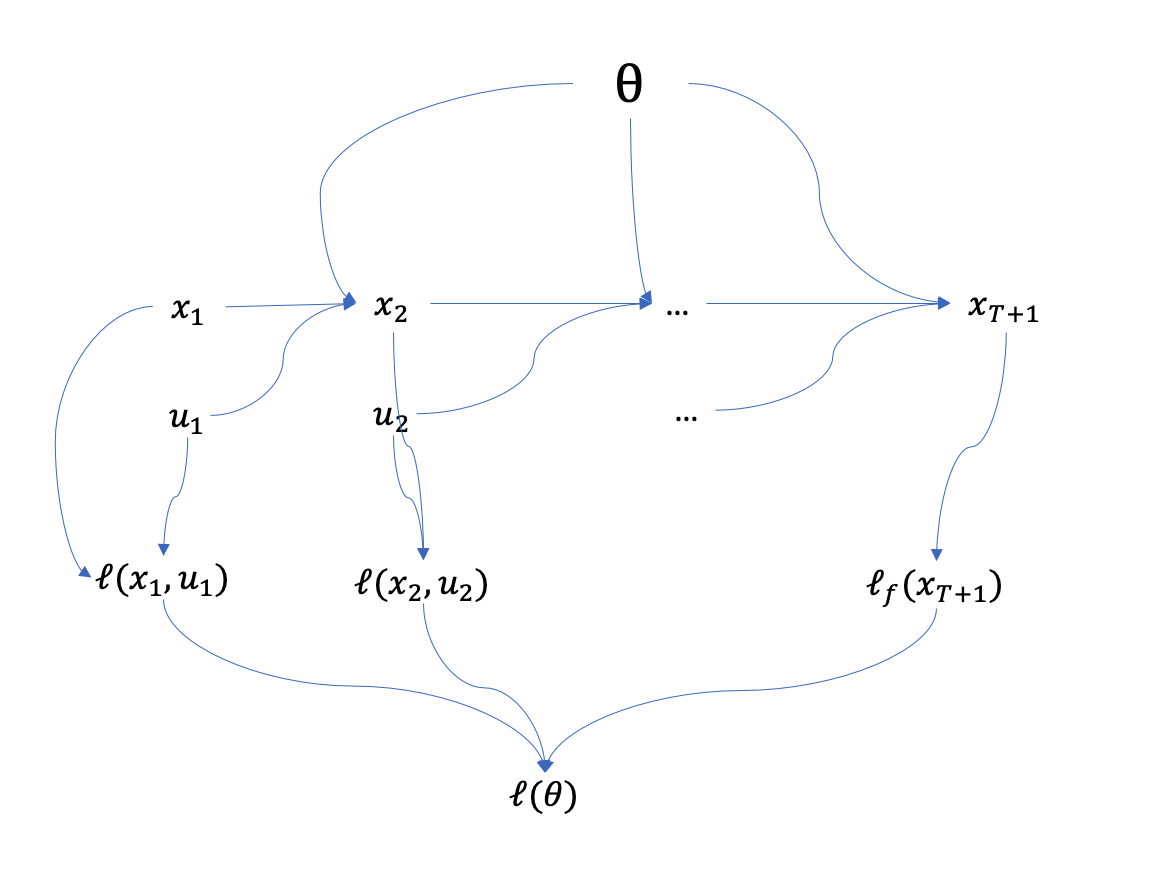
\includegraphics[width=.5\textwidth]{forward_phi.png}
\caption{Forward graph for computing loss}
\end{figure}


\subsection{Model predictive path integral (MPPI) control}
It turns out that Acrobot is not a very easy environment. There are sometimes problems to get the optimal trajectory. Thus we tried also the MPPI method from \cite{williams2017information}. Roughly speaking, for a control sequence $u^i_{1:T}$. The method generates $n$ pertubations $\eps^{1:N}$, then update the control sequence using a scoring system $w$:
\begin{align*}
u_t^{i+1} = u_t^i +  \sum\limits_{n=1}^{N} w(\eps^n) \eps^n_t\,.
\end{align*}
This method does not work very well in general with acrobot.

\subsection{Pendulum}

The acrobot environment is unexpectedly hard to work with, so we tried to work with pendulum first. We consider the dynamics of the pendulum with a damping term $b=1$ as follows:
\begin{align*}
ml^2\ddot{\theta}(t) + mgl \sin \theta(t) = -\dot{\theta}(t) + u(t)
\end{align*}
For a system as easy as pendulum, the method in \ref{subsec:ilqr} works quite well. The method tries to decrease both the mass and the length of the pendulum in order to make the system more controllable. This matches our expectation. 




\section{Experiment and analysis}

\paragraph{Tricks} 
\begin{itemize}
    \item initialization
    \item rk4 
\end{itemize}

\section{Discussion and future works}

\begin{itemize}
    \item Legged robot and contact dynamics
    \item Airplane and aerodynamic
\end{itemize}




\bibliographystyle{IEEEtran}
\bibliography{ref}

\end{document}
